%
% g.tex -- Abbildung der Funktion g
%
% (c) 2023 Prof Dr Andreas Müller
%
\begin{figure}
\centering
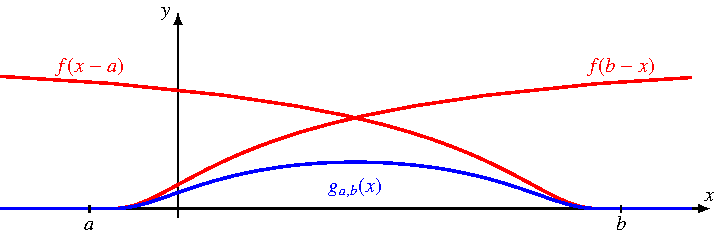
\includegraphics{chapters/020-variation/images/g.pdf}
\caption{Die Funktion $g_{a,b}(x)=f(x-a)f(b-x)$ von
Satz~\ref{buch:variation:fundamentallemma:satz:gab} ist beliebig
oft stetig differenzierbar und hat das offene Intervall $(a,b)$
als Träger $\supp g_{a,b}(x)$.
\label{buch:variation:fundamentallemma:fig:gab}}
\end{figure}
